\chapter[Resultados]{Resultados}
\label{ch:cap4}
%\lipsum[3-5]

Neste capitulo serão apresentados os resultados obtidos e serão feitas algumas observações a respeito desses resultados a partir da modificação do limiar $\alpha$ em sete valores diferentes. Primeiramente, serão apresentados os dados obtidos para cada limiar e após isso será feita a comparação entre os resultados.

\section{Resultados obtidos para diferentes valores do Limiar}
Os resultados apresentados nesta seção foram obtidos a partir da modificação do limiar antes do processo de aprendizagem. Essa modificação é realizada a partir da alteração da consetante $\alpha$ como ja apresentado nos capítulos anteriores deste trabalho.


\subsection{$\alpha$ = 0}
O primeiro experimento realizado foi utilizando o $\alpha$ = 0, ou seja, não é realizada nenhuma poda no modelo. O primeiro experimento foi executado sem poda para futuras comparações entre o modelo otimizado e o não otimizado. Dessa forma, a esparsidade final é igual a 0\%. A partir da Figura 15, é possível ver a variação dos valores de acurácia de treinamento e de validação durante as 30 épocas.

\begin{figure}[H]
    %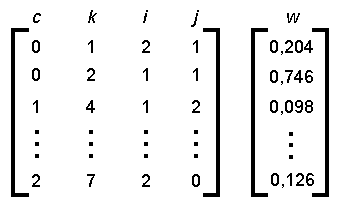
\includepdf[pages=-, width=6cm]{figuras/figx.pdf}
	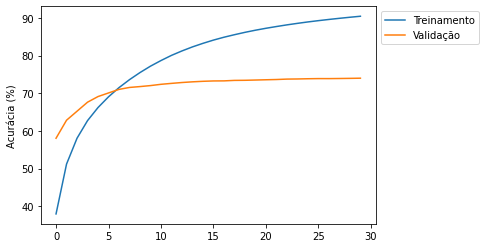
\includegraphics[width=0.6\textwidth, keepaspectratio=true]{figuras/CAP4/acuracia0.png}
	\centering
	\caption[Acurácia de treinamento e validação para $\alpha$ = 0]{Acurácia de treinamento e validação para $\alpha$ = 0}
	\fonte{Elaborada pela autor.}
	%\label{fig:sharpe}
\end{figure}

Para analisar o comportamento dos pesos ao final do treinamento, foi montado um histograma contendo todos os pesos da segunda camada convolucional do modelo, como visto na Figura 16. É possível perceber que uma grande quantidade de pesos se concentram em valores próximos a zero.

\begin{figure}[H]
    %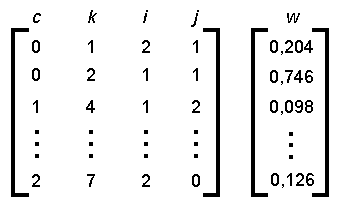
\includepdf[pages=-, width=6cm]{figuras/figx.pdf}
	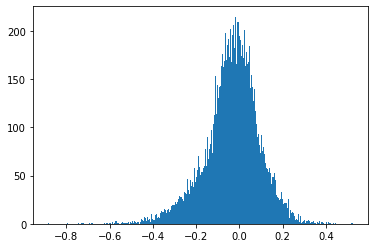
\includegraphics[width=0.5\textwidth, keepaspectratio=true]{figuras/CAP4/hist0_.png}
	\centering
	\caption[Histograma de pesos da segunda camada convolucional do modelo para $\alpha$ = 0]{Histograma de pesos da segunda camada convolucional do modelo para $\alpha$ = 0}
	\fonte{Elaborada pela autor.}
	%\label{fig:sharpe}
\end{figure}

No processo de inferência, obteve-se uma acurácia de 75,30\%. Para visualização dos resultados, a Figura 17 mostra a matriz de confusão obtida. 

\begin{figure}[H]
    %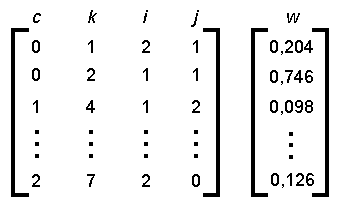
\includepdf[pages=-, width=6cm]{figuras/figx.pdf}
	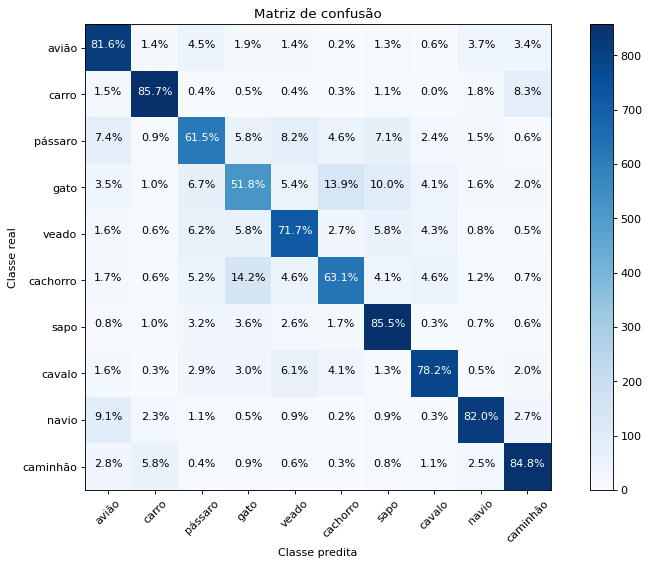
\includegraphics[width=0.7\textwidth, keepaspectratio=true]{figuras/CAP4/cm_0_.png}
	\centering
	\caption[Matriz de confusão para $\alpha$ = 0]{Matriz de confusão para $\alpha$ = 0}
	\fonte{Elaborada pela autor.}
	%\label{fig:sharpe}
\end{figure}


\subsection{$\alpha$ = 0,25}
Após o experimento realizado sem compressão, foi realizado o mesmo processo de treinamento, porém o $\alpha$ foi alterado para 0,25, sendo esse o valor menos agressivo de poda realizado durante todos os experimentos. Dessa vez, o modelo apresentará esparsidade maior que 0\%, uma vez que haverá poda. A Figura 18 mostra a acurácia de e treinamento e validação para o novo valor do limiar. Já a variação da esparsidade durante as épocas pode ser vizualizada na Figura 19. A esparsidade final do modelo chegou a 52,72\%.

\begin{figure}[H]
    %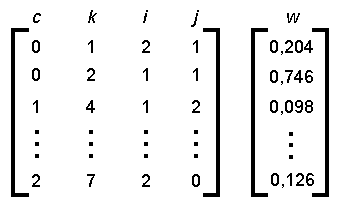
\includepdf[pages=-, width=6cm]{figuras/figx.pdf}
	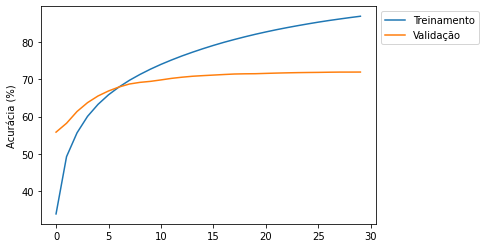
\includegraphics[width=0.6\textwidth, keepaspectratio=true]{figuras/CAP4/acuracia025.png}
	\centering
	\caption[Acurácia de treinamento e validação para $\alpha$ = 0,25]{Acurácia de treinamento e validação para $\alpha$ = 0,25}
	\fonte{Elaborada pela autor.}
	%\label{fig:sharpe}
\end{figure}

\begin{figure}[H]
    %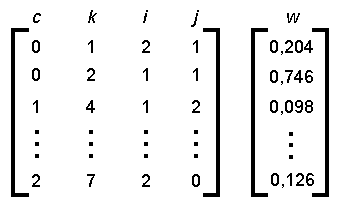
\includepdf[pages=-, width=6cm]{figuras/figx.pdf}
	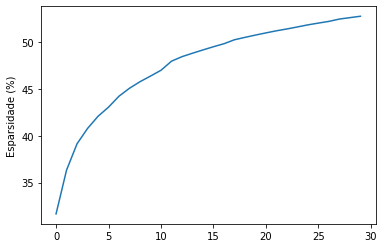
\includegraphics[width=0.5\textwidth, keepaspectratio=true]{figuras/CAP4/esparsidade025.png}
	\centering
	\caption[Variação da esparsidade durante as épocas para $\alpha$ = 0,25]{Variação da esparsidade durante as épocas para $\alpha$ = 0,25}
	\fonte{Elaborada pela autor.}
	%\label{fig:sharpe}
\end{figure}

A Figura 20 contém o histograma dos pesos da segunda camada convolucional. Devido o processo de compressão há uma grande concentração de pesos com valores muito próximos de zero, ou seja, os pesos a serem removidos por não terem grande influência no processo de classificação. Por esse motivo, foi necessário ampliar o histograma para verificar os pesos maiores que o limiar, como apresentado na Figura 21. 


\begin{figure}[H]
	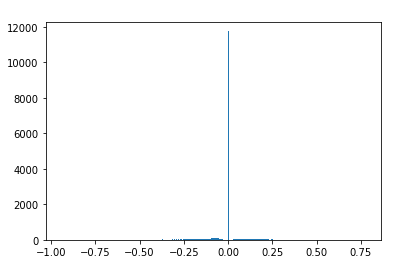
\includegraphics[width=0.5\textwidth, keepaspectratio=true]{figuras/CAP4/hist1_025_.png}
	\centering
	\caption[Histograma de pesos da segunda camada convolucional para $\alpha$ = 0,25]{Histograma de pesos da segunda camada convolucional para $\alpha$ = 0,25}
	\fonte{Elaborada pela autor.}
	%\label{fig:sharpe}
\end{figure}

\begin{figure}[H]
    %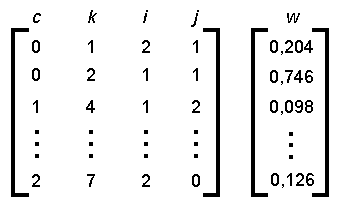
\includepdf[pages=-, width=6cm]{figuras/figx.pdf}
	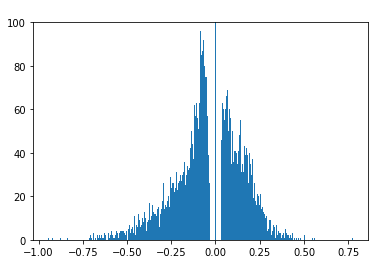
\includegraphics[width=0.5\textwidth, keepaspectratio=true]{figuras/CAP4/hist2_025_.png}
	\centering
	\caption[Histograma ampliado de pesos da segunda camada convolucional para $\alpha$ = 0,25]{Histograma de pesos da segunda camada convolucional para $\alpha$ = 0,25}
	\fonte{Elaborada pela autor.}
	%\label{fig:sharpe}
\end{figure}

No processo de inferência, foi obtida uma acurácia de 73,25\%, ou seja, quando comparado ao modelo não comprimido, é possível remover 52,72\% dos pesos e obter uma acurácia apenas 2,05\% menor. É possível analisar o resultado a partir da matriz de confusão na Figura  22.


\begin{figure}[H]
    %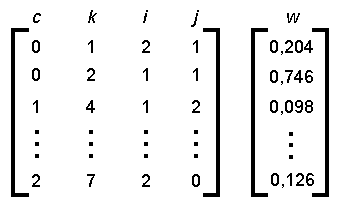
\includepdf[pages=-, width=6cm]{figuras/figx.pdf}
	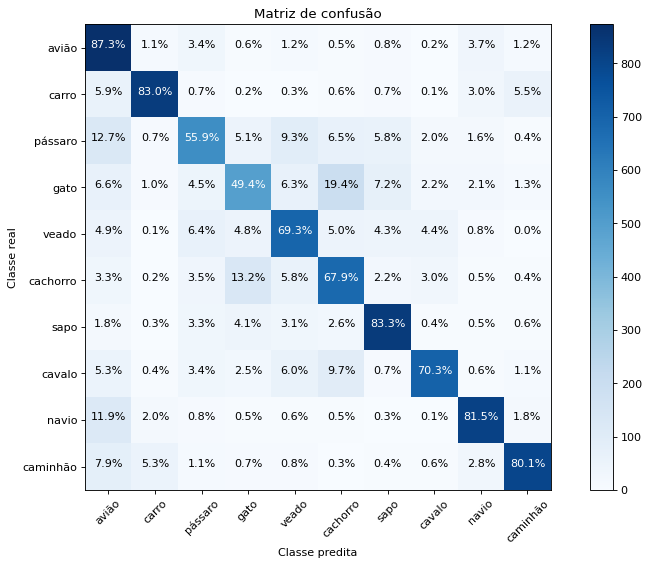
\includegraphics[width=0.68\textwidth, keepaspectratio=true]{figuras/CAP4/cm_025_.png}
	\centering
	\caption[Matriz de confusão para $\alpha$ = 0,25]{Matriz de confusão para $\alpha$ = 0,25}
	\fonte{Elaborada pela autor.}
	%\label{fig:sharpe}
\end{figure}


\subsection{$\alpha$ = 0,50}
O terceiro experimento consistiu em manter o mesmo processo de treinamento e inferência, mas dessa vez alterando o valor de $\alpha$ para 0,50. A Figura 23 apresenta o valor das acurácias de treino e validação para o modelo nessas configurações e a Figura 24 mostra a variação da esparsidade.A esparsidade do modelo chegou a aproximadamente 68,25\%.






\begin{figure}[H]
    %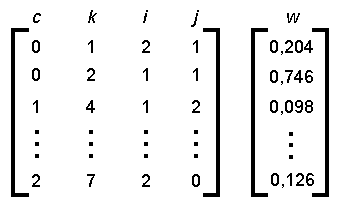
\includepdf[pages=-, width=6cm]{figuras/figx.pdf}
	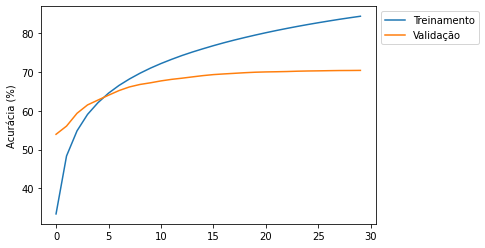
\includegraphics[width=0.6\textwidth, keepaspectratio=true]{figuras/CAP4/acuracia05.png}
	\centering
	\caption[Acurácia de treinamento e validação para $\alpha$ = 0,50]{Acurácia de treinamento e validação para $\alpha$ = 0,50}
	\fonte{Elaborada pela autor.}
	%\label{fig:sharpe}
\end{figure}

Assim como no experimento anterior, foi visualizado o histograma de pesos da segunda camada convolucional. Como a quantidade de pesos próximos a zero foi muito alta, foi impossível analisar os pesos com valores mais altos, em módulo, que o limiar. Portanto, a Figura 25 apresenta o histograma de pesos já ampliado.

Com o fim do treinamento, foi feita a inferência no modelo. O resultado foi uma acurácia de 71,90\%, mostrando que é possível remover aproximadamente 68,25\% dos parâmetros do modelo e obter uma acurácia apenas 3,4\% menor que a do modelo não comprimido. A matriz de confusão pode ser visualizada na Figura 26.

\begin{figure}[H]
    %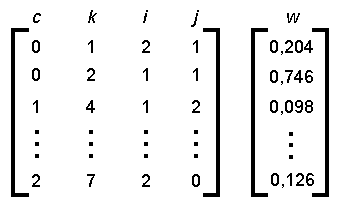
\includepdf[pages=-, width=6cm]{figuras/figx.pdf}
	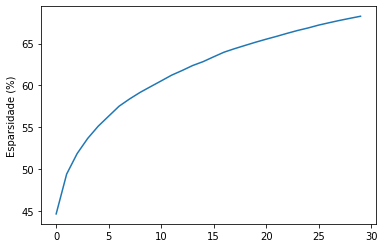
\includegraphics[width=0.5\textwidth, keepaspectratio=true]{figuras/CAP4/esparsidade05.png}
	\centering
	\caption[Variação da esparsidade durante as épocas para $\alpha$ = 0,50]{Variação da esparsidade durante as épocas para $\alpha$ = 0,50}
	\fonte{Elaborada pela autor.}
	%\label{fig:sharpe}
\end{figure}

\begin{figure}[H]
    %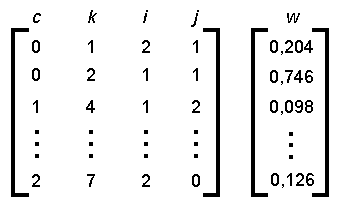
\includepdf[pages=-, width=6cm]{figuras/figx.pdf}
	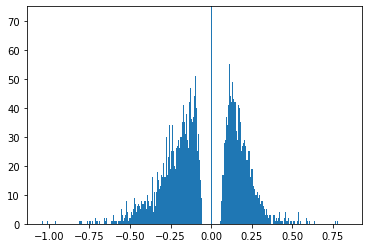
\includegraphics[width=0.5\textwidth, keepaspectratio=true]{figuras/CAP4/hist_50_.png}
	\centering
	\caption[Histograma de pesos da segunda camada convolucional para $\alpha$ = 0,50]{Histograma de pesos da segunda camada convolucional para $\alpha$ = 0,50}
	\fonte{Elaborada pela autor.}
	%\label{fig:sharpe}
\end{figure}

\begin{figure}[H]
    %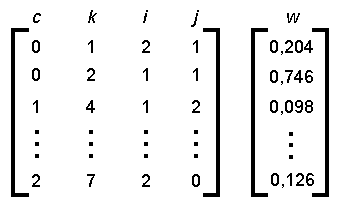
\includepdf[pages=-, width=6cm]{figuras/figx.pdf}
	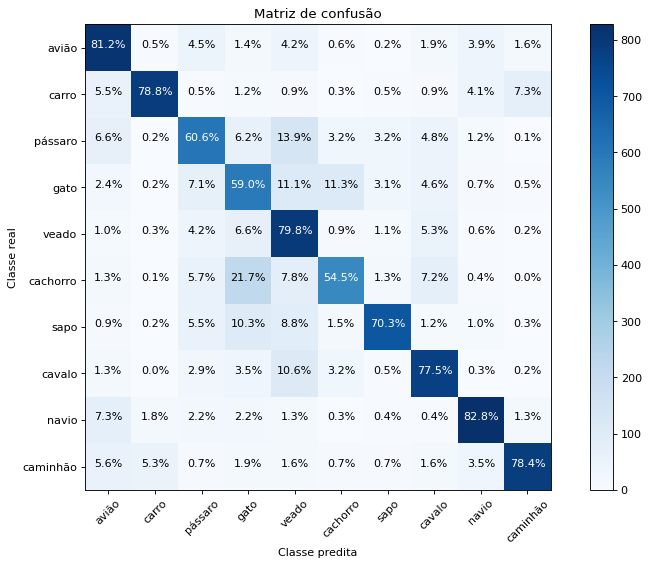
\includegraphics[width=0.65\textwidth, keepaspectratio=true]{figuras/CAP4/cm_05_.png}
	\centering
	\caption[Matriz de confusão para $\alpha$ = 0,50]{Matriz de confusão para $\alpha$ = 0,50}
	\fonte{Elaborada pela autor.}
	%\label{fig:sharpe}
\end{figure}



\subsection{$\alpha$ = 0,75}

Os próximos resultados são obtidos a partir do mesmo procedimento dos experimentos anteriores, porém com $\alpha$ = 0,75. As acurácias de treinamento e validação podem ser observadas na Figura 27 e a variação da esparsidade durante o treinamento pode ser visualizada na Figura 28. A esparsidade final do modelo foi de 82,30\%. O histograma de pesos pode ser visto na Figura 29.


\begin{figure}[H]
    %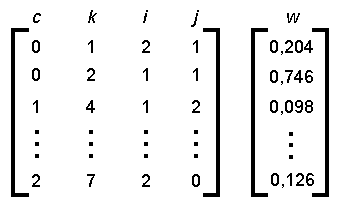
\includepdf[pages=-, width=6cm]{figuras/figx.pdf}
	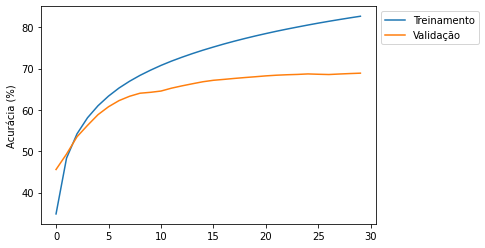
\includegraphics[width=0.6\textwidth, keepaspectratio=true]{figuras/CAP4/acuracia075.png}
	\centering
	\caption[Acurácia de treinamento e validação para $\alpha$ = 0,75]{Acurácia de treinamento e validação para $\alpha$ = 0,75}
	\fonte{Elaborada pela autor.}
	%\label{fig:sharpe}
\end{figure}

\begin{figure}[H]
    %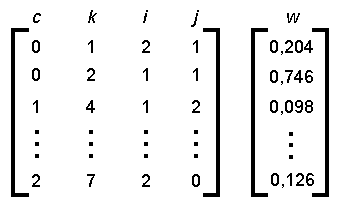
\includepdf[pages=-, width=6cm]{figuras/figx.pdf}
	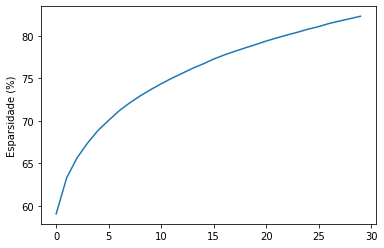
\includegraphics[width=0.5\textwidth, keepaspectratio=true]{figuras/CAP4/esparsidade075.png}
	\centering
	\caption[Variação da esparsidade durante as épocas para $\alpha$ = 0,75]{Variação da esparsidade durante as épocas para $\alpha$ = 0,75}
	\fonte{Elaborada pela autor.}
	%\label{fig:sharpe}
\end{figure}

\begin{figure}[H]
    %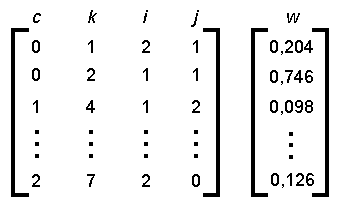
\includepdf[pages=-, width=6cm]{figuras/figx.pdf}
	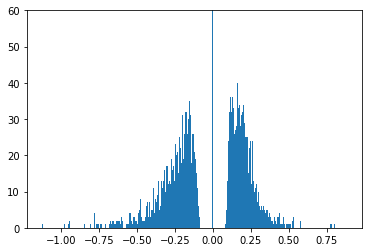
\includegraphics[width=0.5\textwidth, keepaspectratio=true]{figuras/CAP4/hist075_.png}
	\centering
	\caption[Histograma de pesos da segunda camada convolucional para $\alpha$ = 0,75]{Histograma de pesos da segunda camada convolucional para $\alpha$ = 0,75}
	\fonte{Elaborada pela autor.}
	%\label{fig:sharpe}
\end{figure}

Dessa vez, a acurácia de inferência foi de 71,84\%, sendo possível então a remoção de 82,30\% dos parâmetros do modelo para obteção de uma acurácia de inferência apenas 3,46\% menor que a da rede neural não comprimida. A matriz de confusão pode ser visualizada na Figura 30.

\begin{figure}[H]
    %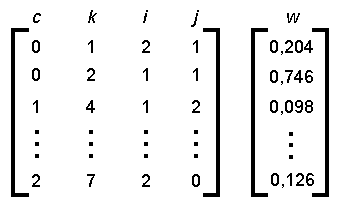
\includepdf[pages=-, width=6cm]{figuras/figx.pdf}
	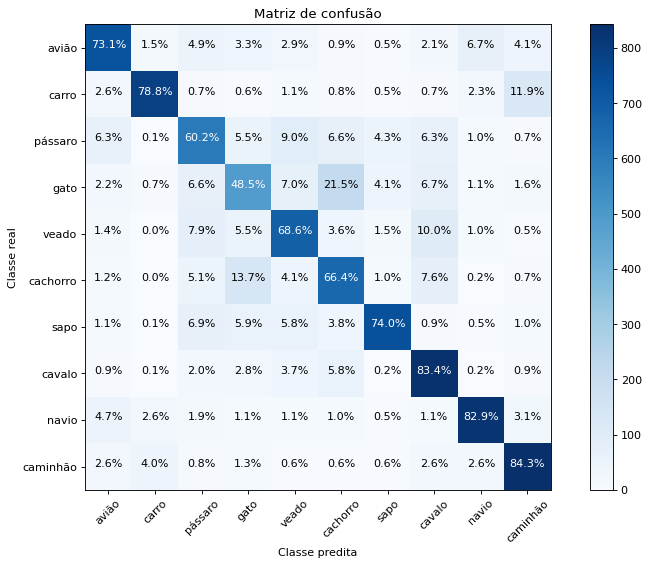
\includegraphics[width=0.65\textwidth, keepaspectratio=true]{figuras/CAP4/cm075_.png}
	\centering
	\caption[Matriz de confusão para $\alpha$ = 0,75]{Matriz de confusão para $\alpha$ = 0,75}
	\fonte{Elaborada pela autor.}
	%\label{fig:sharpe}
\end{figure}




\subsection{$\alpha$ = 1,00}
O próximo experimento foi realizado com o $\alpha$ igual a 1,00. Desta vez o limiar será igual ao desvio padrão da camada. É possível vizualizar as acurácias de treinamento e validação na Figura 31 e a variação da esparsidade na Figura 32. Ao final do processo de aprendizagem, a esparsidade foi de 92,44\%.

\begin{figure}[H]
    %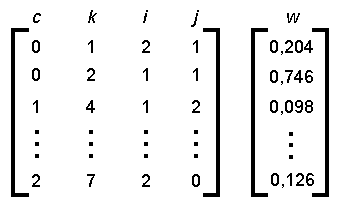
\includepdf[pages=-, width=6cm]{figuras/figx.pdf}
	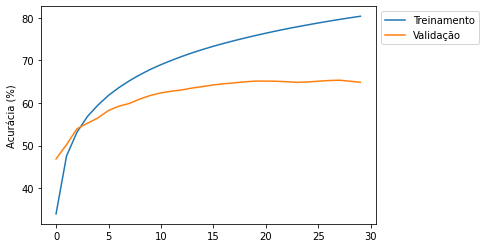
\includegraphics[width=0.6\textwidth, keepaspectratio=true]{figuras/CAP4/acuracia10.png}
	\centering
	\caption[Acurácia de treinamento e validação para $\alpha$ = 1,00]{Acurácia de treinamento e validação para $\alpha$ = 1,00}
	\fonte{Elaborada pela autor.}
	%\label{fig:sharpe}
\end{figure}

A Figura 33 aprensenta o histograma de pesos após o processo de compressão por poda da segunda camada convolucional. A Figura 34 mostra a matriz de confusão da inferência do modelo.

Para este experimento, a acurácia de inferência obtida foi de 67,13\%, sendo então possível obter uma acurácia 7,17\% menor que a do modelo não comprimido ao se remover 92,44\% dos seus parâmetros.

\begin{figure}[H]
    %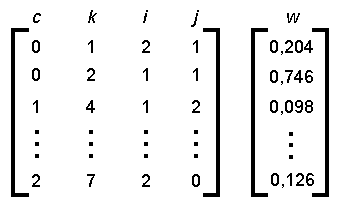
\includepdf[pages=-, width=6cm]{figuras/figx.pdf}
	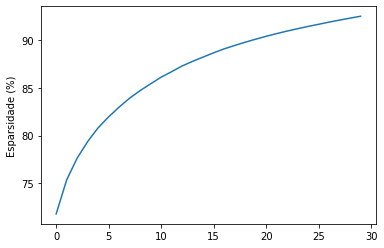
\includegraphics[width=0.5\textwidth, keepaspectratio=true]{figuras/CAP4/esparsidade10.png}
	\centering
	\caption[Variação da esparsidade durante as épocas para $\alpha$ = 1,00]{Variação da esparsidade durante as épocas para $\alpha$ = 1,00}
	\fonte{Elaborada pela autor.}
	%\label{fig:sharpe}
\end{figure}

\begin{figure}[H]
    %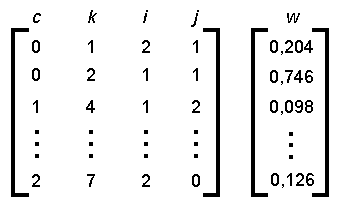
\includepdf[pages=-, width=6cm]{figuras/figx.pdf}
	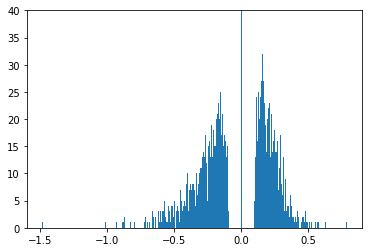
\includegraphics[width=0.5\textwidth, keepaspectratio=true]{figuras/CAP4/hist10_.png}
	\centering
	\caption[Histograma de pesos da segunda camada convolucional para $\alpha$ = 1,00]{Histograma de pesos da segunda camada convolucional para $\alpha$ = 1,00}
	\fonte{Elaborada pela autor.}
	%\label{fig:sharpe}
\end{figure}

\begin{figure}[H]
    %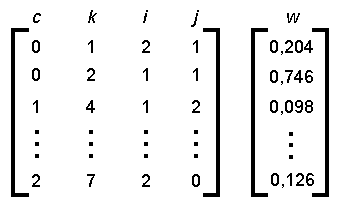
\includepdf[pages=-, width=6cm]{figuras/figx.pdf}
	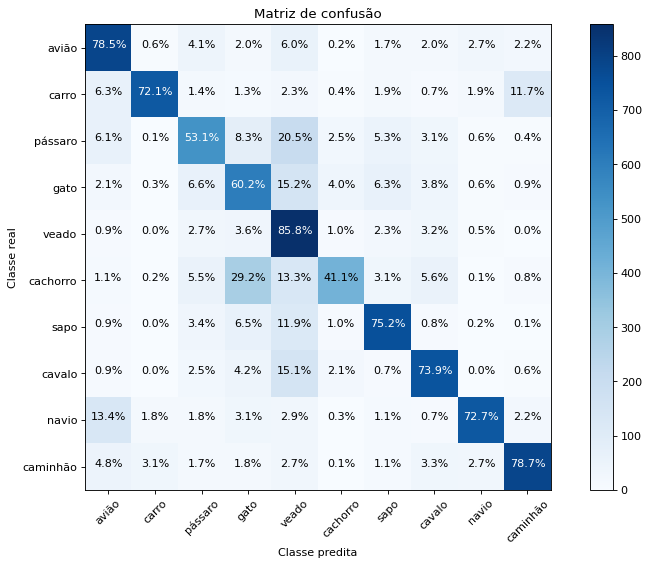
\includegraphics[width=0.65\textwidth, keepaspectratio=true]{figuras/CAP4/cm10_.png}
	\centering
	\caption[Matriz de confusão para $\alpha$ = 1,00]{Matriz de confusão para $\alpha$ = 1,00}
	\fonte{Elaborada pela autor.}
	%\label{fig:sharpe}
\end{figure}


\subsection{$\alpha$ = 1,25}
Neste experimento, o valor de $\alpha$ foi modificado para 1,25 resultando em uma maior agressividade na remoção dos pesos. As acurácias de treinamento e validação podem ser visualizadas na Figura 35, enquanto o comportamento da esparsidade no decorrer do treinamento pode ser visto na Figura 36. A esparsidade chegou a 96,01\%



\begin{figure}[H]
    %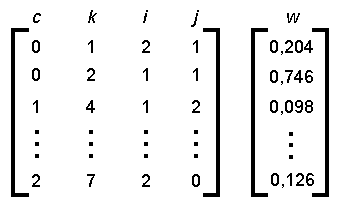
\includepdf[pages=-, width=6cm]{figuras/figx.pdf}
	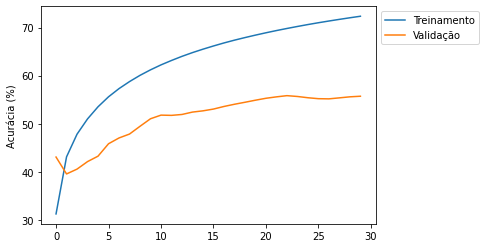
\includegraphics[width=0.6\textwidth, keepaspectratio=true]{figuras/CAP4/acuracia125.png}
	\centering
	\caption[Acurácia de treinamento e validação para $\alpha$ = 1,25]{Acurácia de treinamento e validação para $\alpha$ = 1,25}
	\fonte{Elaborada pela autor.}
	%\label{fig:sharpe}
\end{figure}

Assim como analisado nos experimentos anteriores, foi analisado o histograma de pesos da segunda camada convolucional da rede neural resultante. Assim como já mencionado, foi necessário fazer a ampliação do gráfico de forma que seja possível a visualização dos pesos que não sofreram a poda Este histograma se encontra na Figura 37.

\begin{figure}[H]
    %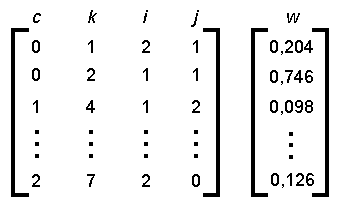
\includepdf[pages=-, width=6cm]{figuras/figx.pdf}
	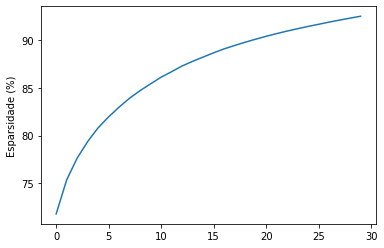
\includegraphics[width=0.5\textwidth, keepaspectratio=true]{figuras/CAP4/esparsidade125.png}
	\centering
	\caption[Variação da esparsidade durante as épocas para $\alpha$ = 1,25]{Variação da esparsidade durante as épocas para $\alpha$ = 1,25}
	\fonte{Elaborada pela autor.}
	%\label{fig:sharpe}
\end{figure}

\begin{figure}[H]
    %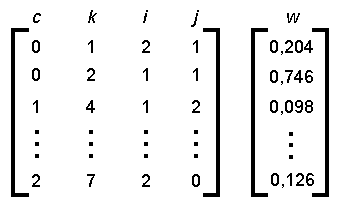
\includepdf[pages=-, width=6cm]{figuras/figx.pdf}
	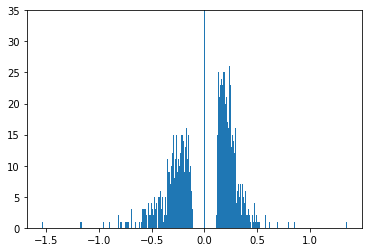
\includegraphics[width=0.5\textwidth, keepaspectratio=true]{figuras/CAP4/hist_125_.png}
	\centering
	\caption[Histograma de pesos da segunda camada convolucional para $\alpha$ = 1,25]{Histograma de pesos da segunda camada convolucional para $\alpha$ = 1,25}
	\fonte{Elaborada pela autor.}
	%\label{fig:sharpe}
\end{figure}

A acurácia de validação do modelo foi de 49,55\%, mostrando que ao se remover paroximadamente 96,01\% dos parâmetros da rede neural em questão, há uma grande interferência na acurácia do modelo, fazendo com que a acurácia de inferência seja 29,75\% menor que a do modelo não comprimido.

Para visualização dos resultados obtidos na inferência, a Figura 38 mostra a matriz de confusão para o modelo. É possível perceber que desta vez a acurácia do modelo foi muito afetada quando o processo de poda foi mais agressivo.

\begin{figure}[H]
    %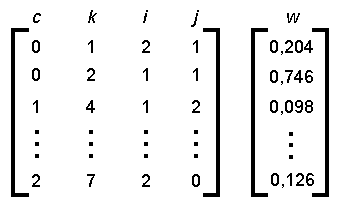
\includepdf[pages=-, width=6cm]{figuras/figx.pdf}
	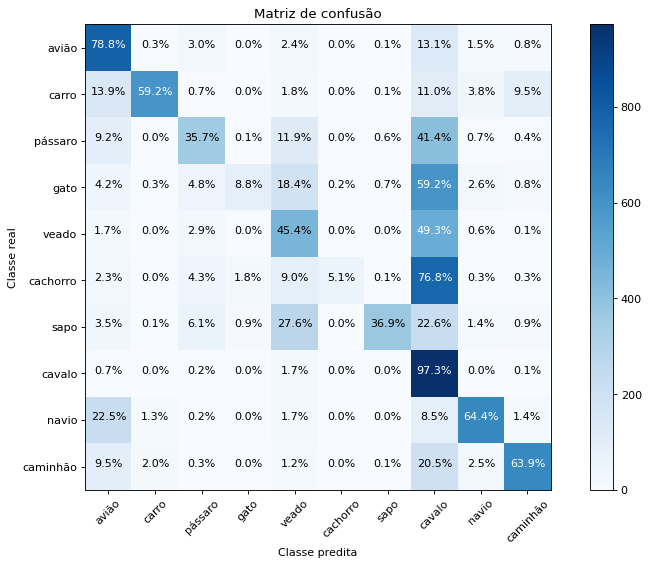
\includegraphics[width=0.65\textwidth, keepaspectratio=true]{figuras/CAP4/cm125_.png}
	\centering
	\caption[Matriz de confusão para $\alpha$ = 1,25]{Matriz de confusão para $\alpha$ = 1,25}
	\fonte{Elaborada pela autor.}
	%\label{fig:sharpe}
\end{figure}



\subsection{$\alpha$ = 1,50}
Como último experimento, o valor de $\alpha$ definido como 1,50. Como resultado, obtive-se o modelo com a maior esparsidade dentre os experimentos anteriores. Pode-se vizualizar as curvas das acurácias de treino e validação na Figura 39 e o comportamento esparsidade durante o treinamento na Figura 40. Ao final do processo de aprendizagem, a esparsidade do modelo chegou a 97,82\%.


\begin{figure}[H]
    %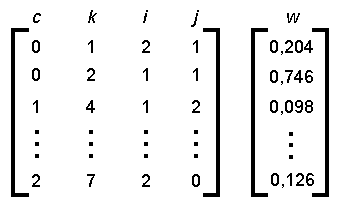
\includepdf[pages=-, width=6cm]{figuras/figx.pdf}
	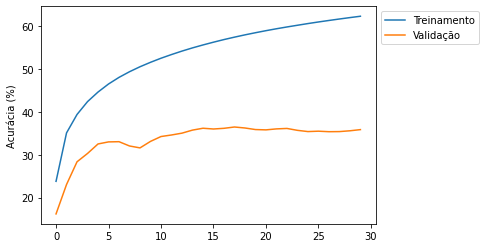
\includegraphics[width=0.6\textwidth, keepaspectratio=true]{figuras/CAP4/acuracia150.png}
	\centering
	\caption[Acurácia de treinamento e validação para $\alpha$ = 1,50]{Acurácia de treinamento e validação para $\alpha$ = 1,50}
	\fonte{Elaborada pela autor.}
	%\label{fig:sharpe}
\end{figure}

O histograma com os pesos da segunda camada convolucional para este experimento pode ser visualizado na Figura 41.

\begin{figure}[H]
    %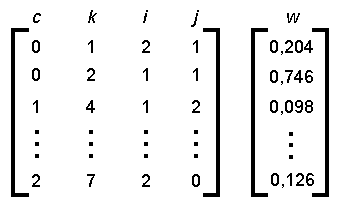
\includepdf[pages=-, width=6cm]{figuras/figx.pdf}
	\includegraphics[width=0.5\textwidth, keepaspectratio=true]{figuras/CAP4/esparsidade150.png}
	\centering
	\caption[Variação da esparsidade durante as épocas para $\alpha$ = 1,50]{Variação da esparsidade durante as épocas para $\alpha$ = 1,50}
	\fonte{Elaborada pela autor.}
	%\label{fig:sharpe}
\end{figure}

\begin{figure}[H]
    %\includepdf[pages=-, width=6cm]{figuras/figx.pdf}
	\includegraphics[width=0.5\textwidth, keepaspectratio=true]{figuras/CAP4/hist_150_.png}
	\centering
	\caption[Histograma de pesos da segunda camada convolucional para $\alpha$ = 1,50]{Histograma de pesos da segunda camada convolucional para $\alpha$ = 1,50}
	\fonte{Elaborada pela autor.}
	%\label{fig:sharpe}
\end{figure}

Para este experimento, a técnica de compressão por poda afetou muito a acurácia da rede. Com a remoção de 97,82\% dos pesos da CNN, a acurácia de validação foi de apenas 44,13\%. A Figura 42 mostra a matriz de confusão deste experimento.


\begin{figure}[H]
    %\includepdf[pages=-, width=6cm]{figuras/figx.pdf}
	\includegraphics[width=0.65\textwidth, keepaspectratio=true]{figuras/CAP4/cm_150_.png}
	\centering
	\caption[Matriz de confusão para $\alpha$ = 1,50]{Matriz de confusão para $\alpha$ = 1,50}
	\fonte{Elaborada pela autor.}
	%\label{fig:sharpe}
\end{figure}



\section{Comparações entre resultados}
Os resultados de acurácia de treinamento e de validação, para os diferentes valores de $\alpha$, podem ser visualizados na Figura 43 (a) e (b), respectivamente. Já o comparativo da variação da esparsidade das redes neurais pode ser visualizado na Figura 43 (c). A Tabela 3 mostra os resultados da esparsidade, acurácia de inferência e número total de parâmetros que não foram removidos para cada valor de $\alpha$. 

\begin{table}[H]
    \centering
    \begin{tabular}{ |p{3cm}|p{3cm}|p{3cm}|p{3cm}|  }
 %\hline
 %\multicolumn{3}{|c|}{} \\
 \hline
 $\alpha$& Esparsidade &Acurácia &Parâmetros\\
 \hline
    0,00        &0,000 \%       &75,300\%    & $\sim$ 1,1M\\
    0,25        &52,728\%       &73,250\%    & $\sim$ 517k\\
    0,50        &68,251\%       &71,900\%    & $\sim$ 347k\\
    0,75        &82,301\%       &71,840\%    & $\sim$ 194k\\
    1,00        &92,465\%       &67,130\%    & $\sim$ 82k\\
    1,25        &96,006\%       &45,550\%    & $\sim$ 44k\\
    1,50        &97,827\%       &44,130\%    & $\sim$ 24k\\
 \hline
\end{tabular}
    \caption{Acurácia e esparsidade dos modelos}
    \label{tab:my_label}
\end{table}

A Figura 44 mostra o comportamento da acurácia de acordo com a esparsidade do modelo. Pode-se observar que a partir de uma certa esparsidade do modelo, a acurácia cai rapidamente devido o limiar englobar os pesos mais significativos da rede. 

Para o modelo em questão, acurácia se manteve acima dos 70\% até a esparsidade de 82,30\%. A partir desse valor a acurácia caí rapidamente, mostrando que a aplicação da técnica de poda de forma muito agressiva gera modelos com baixa acurácia.

\begin{figure}[H]
  \centering
  \subfloat[Acurácias de treinamento]{\includegraphics[width=0.5\textwidth]{figuras/acuracia_geral.png}\label{aaaa}}
  \hfill
  \subfloat[Acurácias de validação]{\includegraphics[width=0.5\textwidth]{figuras/teste_geral.png}\label{bbbb}}
  \hfill
  \subfloat[Esparsidade]{\includegraphics[width=0.5\textwidth]{figuras/sparsity_geral.png}\label{cccc}}
  \hfill
  
  \caption[Comparação entre os resultados dos experimêntos]{Comparação entre resultados dos experimêntos}
  \fonte{Elaborada pela autor.}
\end{figure}

\begin{figure}[H]
    %\includepdf[pages=-, width=6cm]{figuras/figx.pdf}
	\includegraphics[width=0.5\textwidth, keepaspectratio=true]{figuras/accxspar_.png}
	\centering
	\caption[Comparativo das esparsidades]{Comparativo das esparsidades}
	\fonte{Elaborada pela autor.}
	%\label{fig:sharpe}
\end{figure}